\documentclass{beamer}
\mode<presentation>

  \usetheme{Madrid}
  \usecolortheme{default}
  \usefonttheme{default}
  \setbeamertemplate{navigation symbols}{}
  \setbeamertemplate{caption}[numbered]
\usepackage{ragged2e}
\usepackage[english]{babel}
\usepackage[utf8x]{inputenc}
\usepackage{svg}
\usepackage{calc}
\usepackage{amsmath}
\usepackage{subfig}
\usepackage{graphicx}
\graphicspath{ {figures/} }
\setbeamersize{text margin left=0.5cm,text margin right=0.5cm}
\title[SCAD Architecture]{Synchronous Control Asynchronous Dataflow Architecture}
\author{Julius Roob \\ Mahircan G{\"u}l \\ Maisum Haider \\ Subash Kannoth }
\institute[TU Kaiserslautern]
{
	Technische Universit{\"a}t Kaiserslautern \\
	\medskip
}
\date{\today}

\begin{document}

\begin{frame}
  \titlepage
\end{frame}

\begin{frame}[allowframebreaks]{Outline}
\frametitle{Overview}
\tableofcontents
\end{frame}

\section{What is SCAD architecure ?}
  \begin{frame}
  
\end{frame}
  
\section{Instruction set architecture}
  \begin{frame}
  
\end{frame}
  
\section{Move Instruction bus}
  \begin{frame}
\frametitle{Move Instruction Bus (MIB)}
\begin{columns}
	 \begin{column}{0.48\textwidth}
	 		\itemize{
	 			\item \textit{1-to-N} control bus for distributing instructions (from controller to FUs) and transmitting status signals(from FUs to controller)
	 			\item Initial design uses demultiplexer for sending instructions, and multiplexer to encode status signals : N control and status lines
	 			\item Final design uses only one control line for FUs to snoop, however status signals are still transmitted separately (with N lines)
	 		}
	 \end{column}
	 \begin{column}{0.48\textwidth}
	 	\begin{figure}[htbp]
	 		\raggedright
	 		\def\svgscale{0.40}
	 		%%\section{MIB Controller}
	MIB controller is the bridge between control unit and FU network. It establishes communication for both control and status signals, where the former is routed from controller to target and latter is from target to controller, both unidirectionally. Table \ref{table:mib_description} describes input/output ports.  
	
	
	
	\begin{table}[!htbp]
		\begin{tabular}{| l| l | l | p{9cm} |}
			\hline
			\textbf{name} & \textbf{direction} & \textbf{type} &  \textbf{description}\\ \hline
			ctrl & input & mib\_ctrl\_out & control packet from controller. \emph{dest.fu} signal is used to select target. ctrl signal is steered to destination port without modification. \\ \hline
			stat & output & mib\_stalls & status packet from target. \emph{dest.fu} signal of \emph{ctrl} determines the address of target in which its status to be read.  \\ \hline
			mib\_ctrl & output & mib\_ctrl\_bus & control signal group. Every FU in network is connected to the bus in ascending order of their addresses.   \\ \hline
			mib\_stat & input & mib\_status\_bus & status signal group. Status output of FUs in network is connected through corresponding signal   \\ \hline
			
		\end{tabular}
		
		\caption{MIB ports \label{table:mib_description}}
		\centering
	\end{table}
	 
	
	Assuming target address $N$, Figures \ref{fig:ctrl_to_target} and \ref{fig:status_from_target} illustrate control and status packet transfers from controller to target, and from target to controller, respectively. Since availability of both source and destination is checked by controller before performing control operations, packet is held at the bus for a cycle duration only. 
	
	\begin{figure}[!h]
	\centering
	\subfloat[Control packet to target] {
			\begin{tikztimingtable}[timing/lslope=0]
				clk & 14{C} \\
				ctrl.valid & 3L2H9L \\
				ctrl.dest & 3X8D{$N$}3X \\
				ctrl.phase & 3X8D{COMMIT}3X \\
				mib\_ctrl[$N$] & 5X2D{ctrl}7X \\
				mib\_ctrl.valid[$N$] & 5L2H7L \\
			\end{tikztimingtable}
			\label{fig:ctrl_to_target}
		}
			%\caption{Control packet to target}
			%\centering
%	\end{subfloat}
	\hfill
	\subfloat[Status packet from target] {
			\begin{tikztimingtable}[timing/lslope=0]
				clk & 14{C} \\
				ctrl.valid & 3L2H9L \\
				ctrl.dest & 3X8D{$N$}3X \\
				ctrl.phase & 3X8D{CHECK}3X \\
				mib\_stat[$N$] & 5X2D7X \\
			\end{tikztimingtable}
			\label{fig:status_from_target} 
		}
			%\caption{Status packet from target}
			%\centering
	
	\caption{Control and status packet transfer}
	\end{figure}
	
		Design is straightforward, consisting of $1\times\nrFUS$ de-multiplexer for controller to network routing and $\nrFUS\times 1$ multiplexer for opposite direction. Target functional unit is selected by destination address field of MIB control input, regardless of the operation type.  Due to lack of tri-state ic in FPGA fabric to be used, there is many-to-one relationship for status signals between functional units and control unit. Output of every unit is encoded in bus controller using destination address from control unit as line select. However, the opposite is not necessarily true, since a single line from controller for control packages can be snooped by functional units. For simplicity, we prefer using separate lines for control messages as well, by steering packet from controller to target line using destination address as line select. Bus snooping for control messages will be featured after validating main functionality. Figure \ref{fig:mib} shows structure of bus controller.
	\begin{figure}[!htbp]
		\centering
		\def\svgscale{0.50}
		%%\section{MIB Controller}
	MIB controller is the bridge between control unit and FU network. It establishes communication for both control and status signals, where the former is routed from controller to target and latter is from target to controller, both unidirectionally. Table \ref{table:mib_description} describes input/output ports.  
	
	
	
	\begin{table}[!htbp]
		\begin{tabular}{| l| l | l | p{9cm} |}
			\hline
			\textbf{name} & \textbf{direction} & \textbf{type} &  \textbf{description}\\ \hline
			ctrl & input & mib\_ctrl\_out & control packet from controller. \emph{dest.fu} signal is used to select target. ctrl signal is steered to destination port without modification. \\ \hline
			stat & output & mib\_stalls & status packet from target. \emph{dest.fu} signal of \emph{ctrl} determines the address of target in which its status to be read.  \\ \hline
			mib\_ctrl & output & mib\_ctrl\_bus & control signal group. Every FU in network is connected to the bus in ascending order of their addresses.   \\ \hline
			mib\_stat & input & mib\_status\_bus & status signal group. Status output of FUs in network is connected through corresponding signal   \\ \hline
			
		\end{tabular}
		
		\caption{MIB ports \label{table:mib_description}}
		\centering
	\end{table}
	 
	
	Assuming target address $N$, Figures \ref{fig:ctrl_to_target} and \ref{fig:status_from_target} illustrate control and status packet transfers from controller to target, and from target to controller, respectively. Since availability of both source and destination is checked by controller before performing control operations, packet is held at the bus for a cycle duration only. 
	
	\begin{figure}[!h]
	\centering
	\subfloat[Control packet to target] {
			\begin{tikztimingtable}[timing/lslope=0]
				clk & 14{C} \\
				ctrl.valid & 3L2H9L \\
				ctrl.dest & 3X8D{$N$}3X \\
				ctrl.phase & 3X8D{COMMIT}3X \\
				mib\_ctrl[$N$] & 5X2D{ctrl}7X \\
				mib\_ctrl.valid[$N$] & 5L2H7L \\
			\end{tikztimingtable}
			\label{fig:ctrl_to_target}
		}
			%\caption{Control packet to target}
			%\centering
%	\end{subfloat}
	\hfill
	\subfloat[Status packet from target] {
			\begin{tikztimingtable}[timing/lslope=0]
				clk & 14{C} \\
				ctrl.valid & 3L2H9L \\
				ctrl.dest & 3X8D{$N$}3X \\
				ctrl.phase & 3X8D{CHECK}3X \\
				mib\_stat[$N$] & 5X2D7X \\
			\end{tikztimingtable}
			\label{fig:status_from_target} 
		}
			%\caption{Status packet from target}
			%\centering
	
	\caption{Control and status packet transfer}
	\end{figure}
	
		Design is straightforward, consisting of $1\times\nrFUS$ de-multiplexer for controller to network routing and $\nrFUS\times 1$ multiplexer for opposite direction. Target functional unit is selected by destination address field of MIB control input, regardless of the operation type.  Due to lack of tri-state ic in FPGA fabric to be used, there is many-to-one relationship for status signals between functional units and control unit. Output of every unit is encoded in bus controller using destination address from control unit as line select. However, the opposite is not necessarily true, since a single line from controller for control packages can be snooped by functional units. For simplicity, we prefer using separate lines for control messages as well, by steering packet from controller to target line using destination address as line select. Bus snooping for control messages will be featured after validating main functionality. Figure \ref{fig:mib} shows structure of bus controller.
	\begin{figure}[!htbp]
		\centering
		\def\svgscale{0.50}
		\input{figures/mib.pdf_tex}
		\caption{MIB structure}
		\label{fig:mib} 
	\end{figure}
		\caption{MIB structure}
		\label{fig:mib} 
	\end{figure}
	 		\caption{MIB structure}
	 		\label{fig:mib} 
	 	\end{figure}
	 \end{column}
\end{columns}

\end{frame}

  
\section{Control Unit}
  \begin{frame}
  
\end{frame}
  
\section{Data trasport network - DTN}
  \begin{frame}
\frametitle{Data Transport Network}
  \itemize{
    \item DTN is the core part of SCAD \\
    \item Intention is to acheive low latency in deliveing \textit{Data-Packets} from a source \textit{Function-Unit} to destination \textit{Function-Unit}  \\
    \item Low latency means the time taken for deliveing \textit{Data-Packets} is expected to be constant , ie; independent of \textit{Function-Unit} address permuations \\
    \item Many possible solutions\\
     \itemize{
      \item Memory mapped buses - Best in terms of resource but worst in latency\\
      \item Cross Bar switch - Worst in terms of resources but best in terms of latency\\
      \item Parllel sorting Networks like Bitonic Sorter , Benes Network etc - Tradeoff between latency and resource\\
     }
     \item We selected a Bitonic sorter and Benes network.
  }
\end{frame}
  
  \subsection{Bitnoic Network}
    \begin{frame}[shrink=15]%[allowframebreaks]{Outline}
\frametitle{Bitonic network}
  \itemize{
    \item A Bitonic Sort is a comparison based parallel sorting algorithm. \\
    \item A random input sequence in first converted into monotonically increasing and then decreasing thus the name Bitonic - \textit{Bitonic split} \\
    \item A \textit{Bitonic merge} converts Bitonic sequence to sorted sequence. \\
    \item Formally the alogorthim can be expressed as below \\
			      Let \[ 
				  S = \langle x_0,x_1,..x_{n-1}\rangle 
				\] be Bitonic sequence such that
				\[
				    x_0 \leq x_1 \leq ... \leq x_{n/2-1} \quad \textrm{and} \quad  x_{n/2} \leq x_{n/2+1} \leq ... \leq x_{n-1}  \quad \textrm{holds}
				\]
			    Consider the following subsequences
				\[
				  S_{1} =  \langle min(x_0,x_{n/2}), min(x_1,x_{n/2+1}),..,min(x_{n/2-1},x_{n-1})\rangle
				\]
				\[
				  S_{2} =  \langle max(x_0,x_{n/2}), max(x_1,x_{n/2+1}),..,max(x_{n/2-1},x_{n-1})\rangle
				\]
			    with
				\[
				  \forall _{x} \forall _{y}. x \in S_{1}  \wedge  y \in S_{2} \quad x < y
				\]
  }
  \item S1 and S2 recursively yields a sorted sequence.
  \item For $N$ the number of items to be sorted a Bitoni Sorter has $O(N.log_{2}(N))$ stages and a depth of $O(N.log_{2}(N)^{2})$ \\

\end{frame}
    \begin{frame}[shrink=15]
\frametitle{Bitonic network II}
  A 16 input Bitonic Sorter configuration is shown in the Figure below 
 \begin{figure}[!ht]
 \includegraphics[width=11cm, height=7cm]{figures/BitonicSorter16}
 \caption{A 16 input Bitonic sorter}
 \end{figure}
\end{frame}

    
     \subsection{Challenges with Bitnoic Network}
	\begin{frame}
\frametitle{Bitonic network challenges}
 \begin{itemize}
    \item Bitonic network is a sorter not a Router.\\
    \item Can malfunction when some of the inputs have not produced a valid \textit{Data-Packet}. \\
    \item Possibly result in routing \textit{Data-Packet} to wrong target \textit{Function-Units}. \\
    \item Two solutions were identified.\\
    \begin{enumerate}{
	\item Bitnoic Network with Routers \\
	\item Bitonic-Banyan Network \\
    }
    \end{enumerate}
  \end{itemize}
\end{frame}
	
	\subsubsection{Bitnoic Network with Routers}
	\begin{frame}[allowframebreaks]{Outline}
\frametitle{Bitonic Network with Routers}
 \itemize{
    \item All the invalid addresses are removed from the input sequence before feeding to Bitonic sorter.\\
    \item An \textit{Address-Resovler} module is introduced for all the inputs\\
    \item The \textit{Address-Resovler} replaces the invalid addresses by $N -1 + C$, where $C$ is position of the comparator ranges from $1$ to $N$ \\
    \item The Bitonic sorter sorts the sequence and all the invalid inputs comes at the end of sorted sequence\\
    \item The Figure below shows the \textit{Address-Resovler} \\
     \begin{figure}[!ht]
      \includegraphics[width=11cm, height=4.5cm]{figures/Address_Resolver}
      \caption{Address Resovler}
     \end{figure}
  }
  \item The sorted sequence will be the ascending order , but still can reach to wrong destinations. \\
  \item For eg: If the input is an address sequence $\langle31,X_{1},X_{2},..,X_{31}\rangle$ (where $X_{i}$ indicates invalid address) which results in the sorted output sequence 
					      of $\langle31,32,33,..,63\rangle$. The routing is wrong since the $31$ is routed to target $0$ \\
  \item This is indeed a problem since it demands all the inputs to be valid or any permutations of cosecutive input sequence starts with $0$. For eg :  $\langle 0,1,2,3..\rangle$ or $\langle 0,2,3,1..\rangle$ etc\\
  \item This is solved by using a stage of 32 sequencial Routers \\
  \item The configuration is shown in the Figure below.\\
   \begin{figure}[!ht]
    %\includegraphics[width=8.35cm, height=7cm]{figures/RouterNetwork}
    \includegraphics[width=5.2cm, height=4.2cm]{figures/RouterNetwork}
    \caption{Routers at the final stage to reroute to the target}
  \end{figure}
   \item The Routers determine and shortest path from the hardcoded routing table and forwards to the correct neighbours.\\
  \item In the worst case the time taken for a packet to deliver to destination is $N / 2$ clock cycles\\
  \item The best case is one clock cycle when the DTN has all the inputs ready to be routed $N / 2$\\
  \item Drawback - A \textit{stall} is requried until the packet is delivered to the right destination \\
\end{frame} 

      
	\subsubsection{Bitnoic-Banyan Network}
	\begin{frame}[allowframebreaks]{Outline}
\frametitle{Bitonic Banyan Network}
 \begin{itemize}
  \item Self routing property of a Bitonic-Banyan network \\
  \item Configuration contians a Bitonic network cascased with a Banyan Tree. \\
  \item Bitonic network configuration remains the same except the switches are modified. \\
  \item Below are the different scenarios for the modified switches\\
   \begin{figure}[!ht]
    %\includegraphics[width=8.35cm, height=7cm]{figures/RouterNetwork}
    \includegraphics[width=7cm, height=2cm]{figures/Batcher_Switches}
    \caption{Modified switches for Bitonic network }
  \end{figure}
  \item The \textit{Normal switch} and \textit{Modified switch} are mutliplexed w.r.t the \textit{VALID} bit.
  \item The below figure shows the implemention of switching element.
  \begin{figure}[!ht]
    %\includegraphics[width=8.35cm, height=7cm]{figures/RouterNetwork}
    \includegraphics[width=7cm, height=3.5cm]{figures/Switching_Element}
    \caption{Swithing element of Bitonic Network}
  \end{figure}
  \item A N input Banyan network characterized of $O( N.log_{2}(N)$ switching elements and $O(log_{2}(N)$ stages \\
  \item A Banyan switch routes the input based on the $i^{th}$ bit of the header. In our case the \textit{Target-Address} \\
  and  $i$ is the index of the Banyan stage.
  \item In our case to handle the invalid addresses, the bit controlled algorithm is modified as shown in the following figure \\
   \begin{figure}[!ht]
    %\includegraphics[width=8.35cm, height=7cm]{figures/RouterNetwork}
    \includegraphics[width=9cm, height=0.8cm]{figures/Banyan_Switches}
    \caption{ Different senarios of a banyan switch}
  \end{figure}
  \item  A Banyan newtwork is always collision free if the input sequences are sorted ascending.\\
  \item  The initial Bitnoic stage ensures ascending sequence at the input of the Banyan thus gurantee a collision free Banyan network. \\
  \item  The below figures depicts a screen capture of the VHDL Simulation\\
   \begin{figure}[!htb]
  \minipage{0.32\textwidth}
  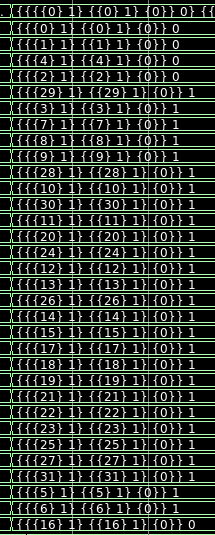
\includegraphics[width=2.2 cm, height=5.5cm]{figures/1}
  \caption{Input sequence}
  \endminipage\hfill
  \minipage{0.32\textwidth}
  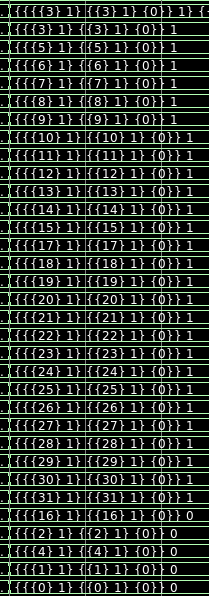
\includegraphics[width=2.2 cm, height=5.5 cm]{figures/2}
  \caption{After Bitonic stage}
  \endminipage\hfill
  \minipage{0.32\textwidth}%
  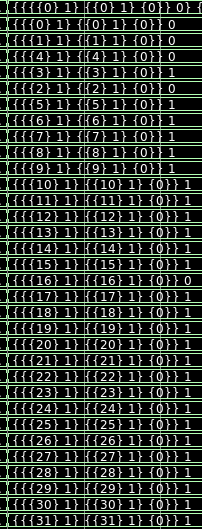
\includegraphics[width=2.2cm, height=5.5cm]{figures/3}
  \caption{After Banyan tree}
  \endminipage
  \end{figure}
  \item From benchmarks its has been already proven tha for $N > 8$ the latency due to combinatorial depth of a Bitonic network is more that when it is piplelined.\\
  \item Implemented 5 stage pipleline for th Bitonic network also a 5 stage pipeline for the Banyan network.\\
  \item The complete design of the DTN is shown as below. \\
    \begin{figure}[!ht]
    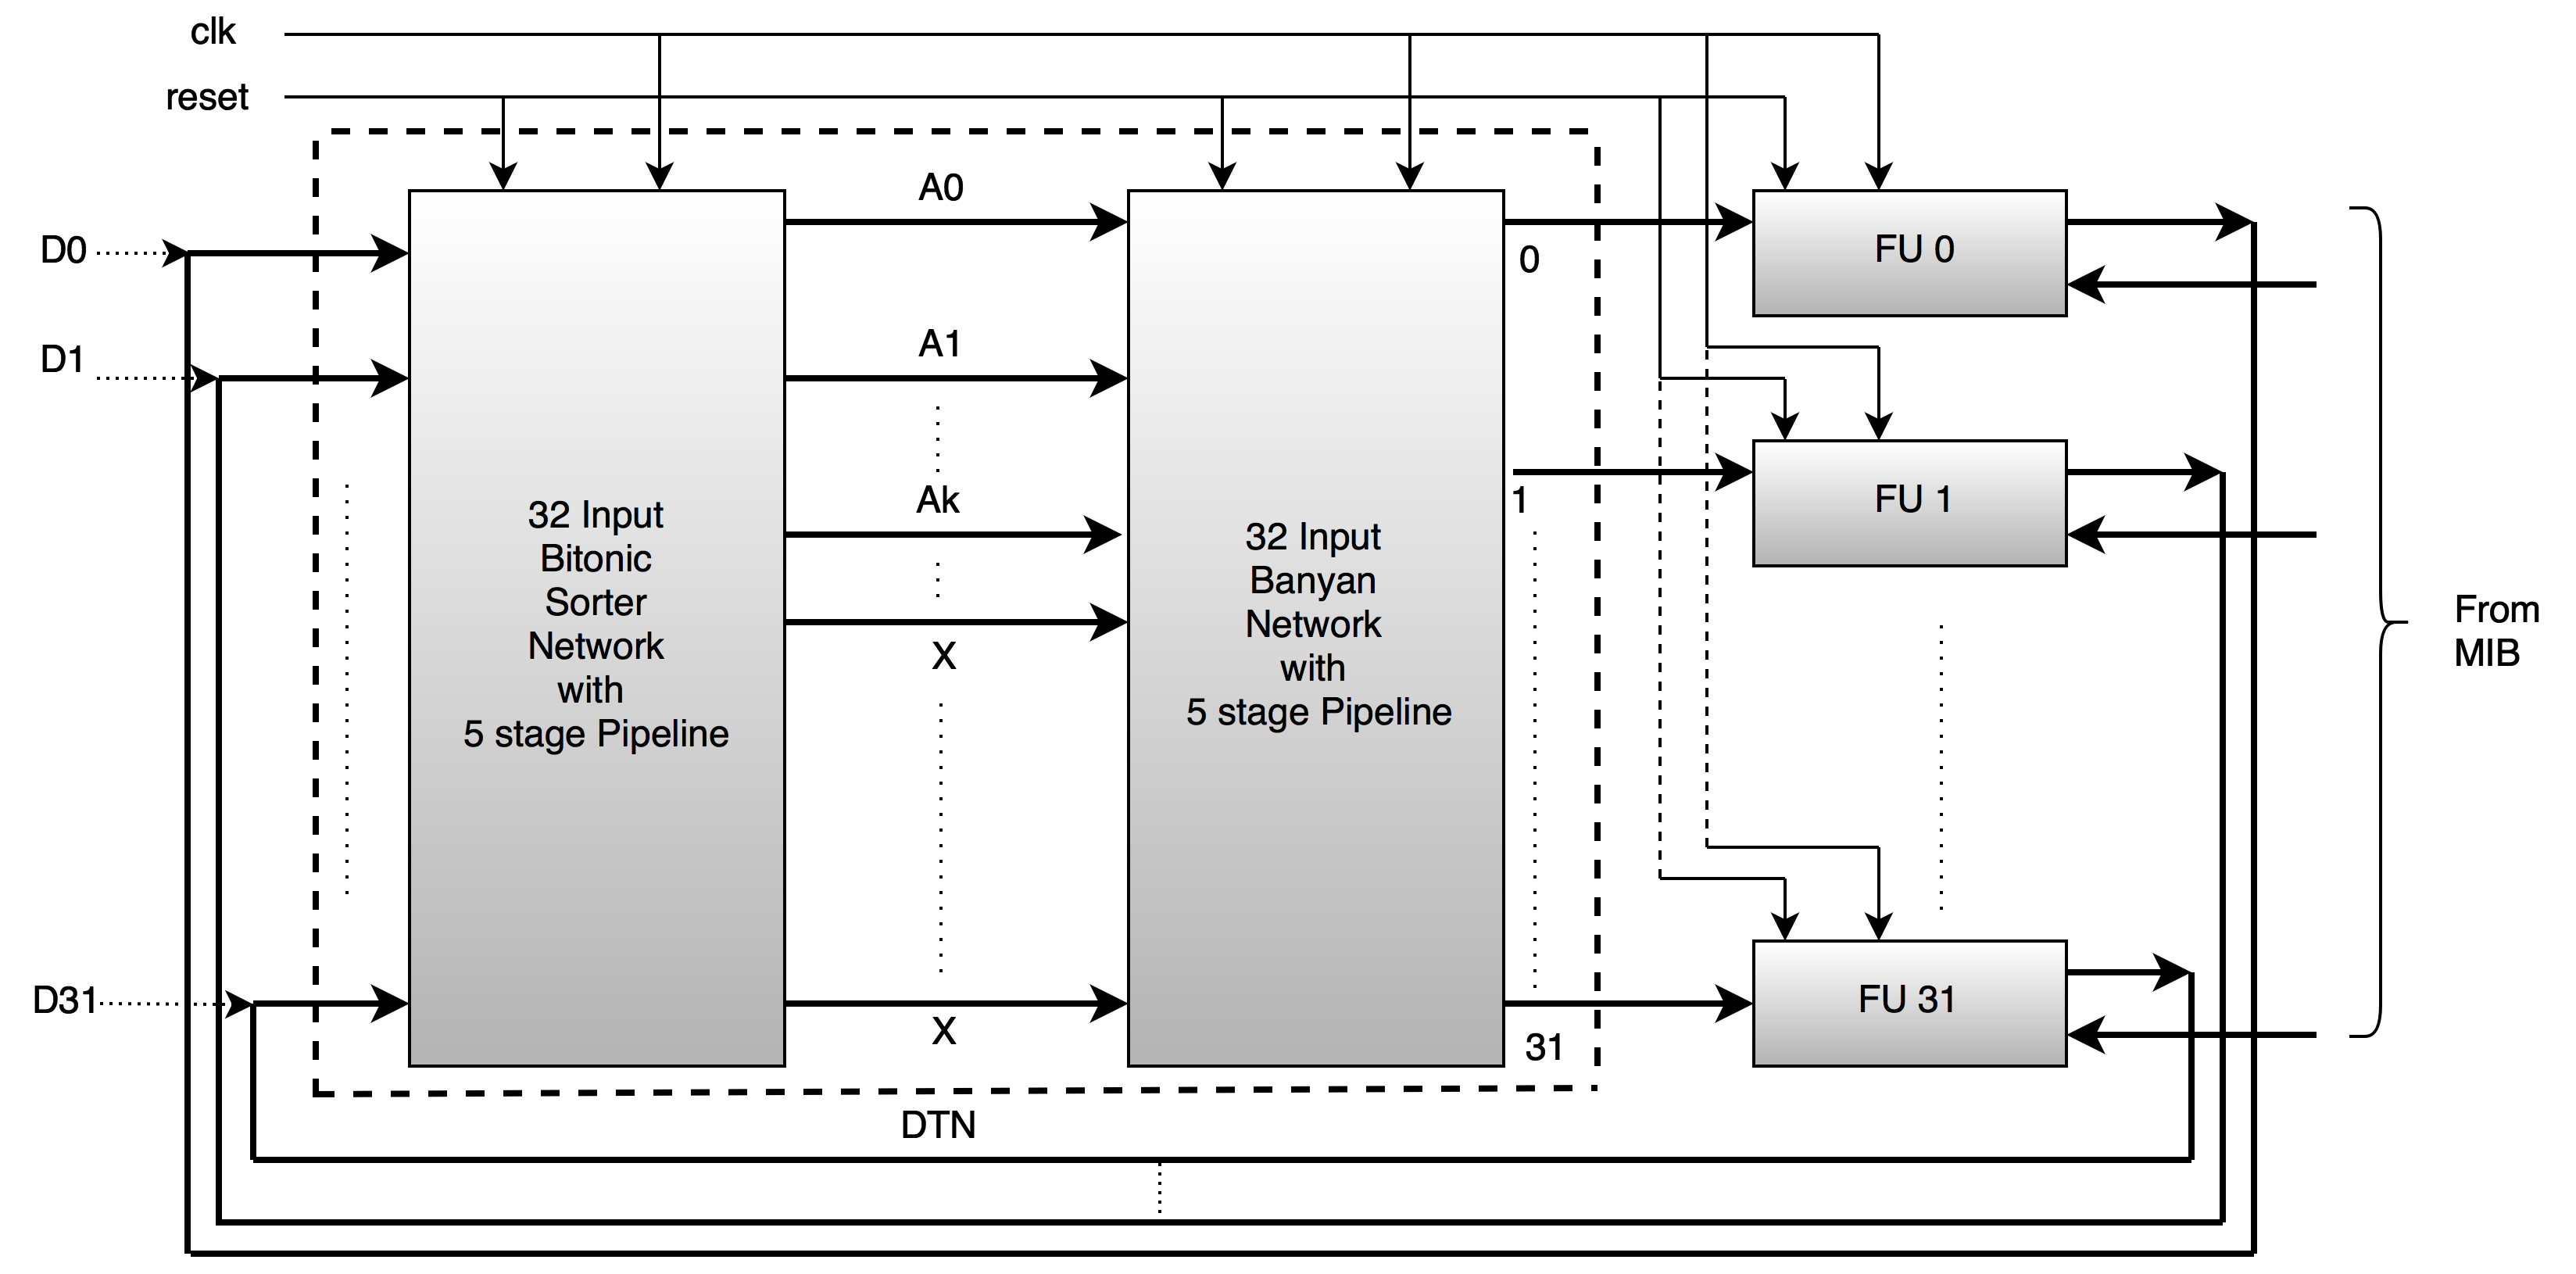
\includegraphics[width=9cm, height=5cm]{figures/Batcher_Banyan_Combined}
    \caption{Bitnoic-Banyan DTN of SCAD architecture}
  \end{figure}
  \end{itemize}
\end{frame}

	
	\subsubsection{Resource Utilization}
	  \begin{frame}[shrink=20]
\frametitle{Resource utilization}

\begin{table}
  \begin{tabular}{l | c | c }
     \textbf{Site Type}  & \textbf{Bitnoic with routers (\%)} & \textbf{Bitnoic-Banyan(\%)} \\
    \hline \hline
    Slice LUTs 			& 30.85 & 37.65 \\ 
    \quad LUT as Logic		& 30.85 & 37.65 \\
    \quad LUT as Memory		& 0.00 & 0.00 	\\
    Slice Registers 		& 11.12	& 13.53 \\
    \quad Register as Flip Flop	& 11.12	& 13.53	\\
    \quad Register as Latch	& 0.00	& 0.00	\\
    F7 Muxes			& 0.00	& 0.00	\\
    F8 Muxes 			& 0.00	& 0.00	\\
  \end{tabular}
  \caption{Resource utilization of DTN with Bitnoic network}
\end{table}
\itemize{
  \item The total utilization for sequencial implementation with routers 41.92\%
  \item The total utilization for complete parallel implementation with Bitnoic-Banyan 51.18\%
  \item As a tradeoff between resource utilization and time to deliver a Data-Packet Bitnoic-Banyan is a better choice
}

\end{frame}
      
  \subsection{Benes Network}
		\begin{frame}
	\frametitle{Benes Network}
	\begin{center}
		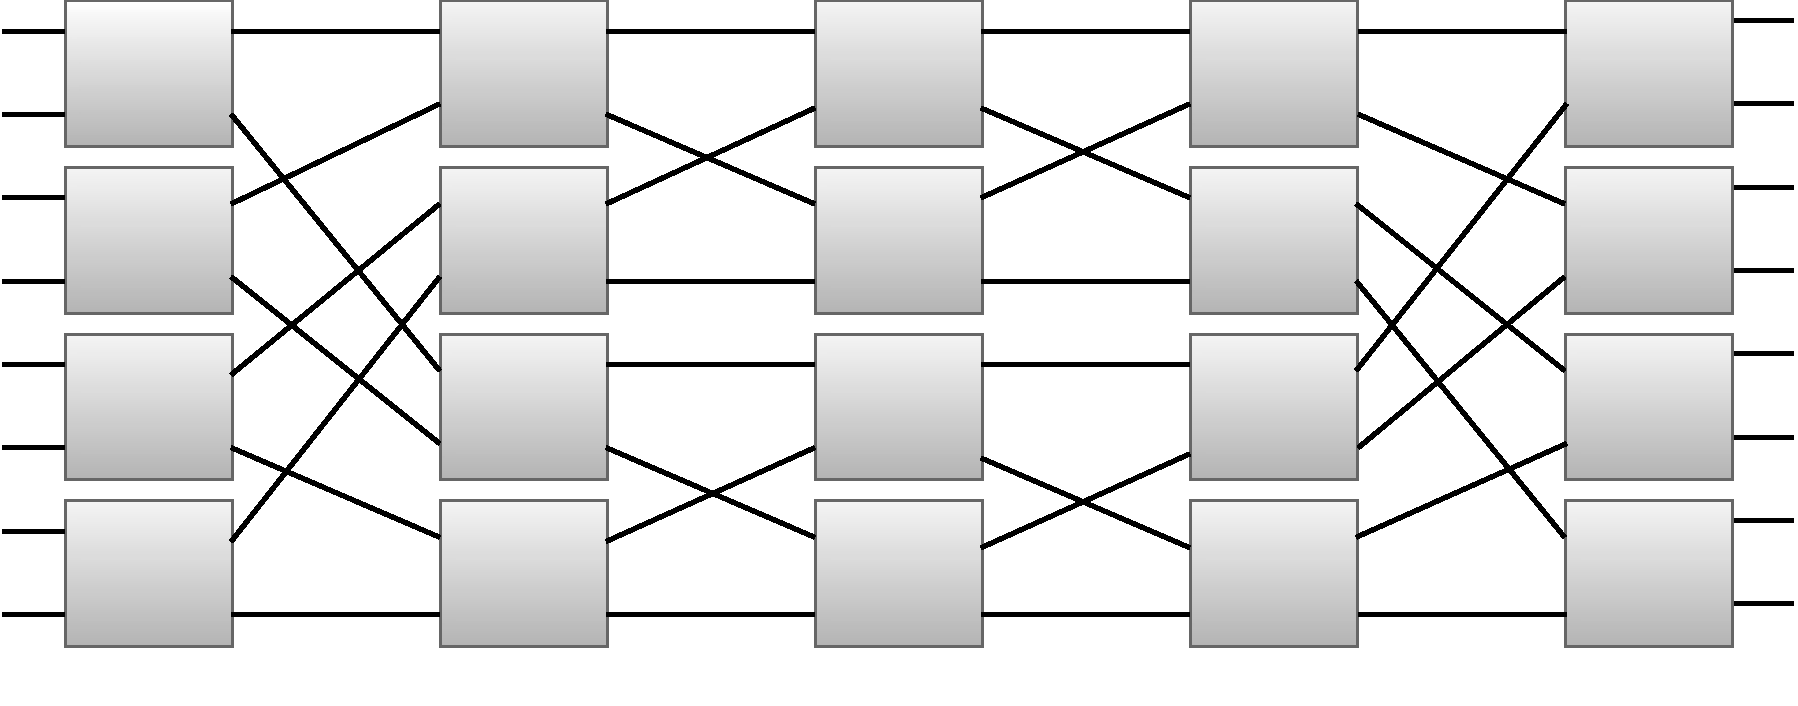
\includegraphics[width=0.9\linewidth]{benes_network.pdf}
	\end{center}
\end{frame}

\begin{frame}
	\frametitle{Benes Network: Recursion}
	\begin{center}
		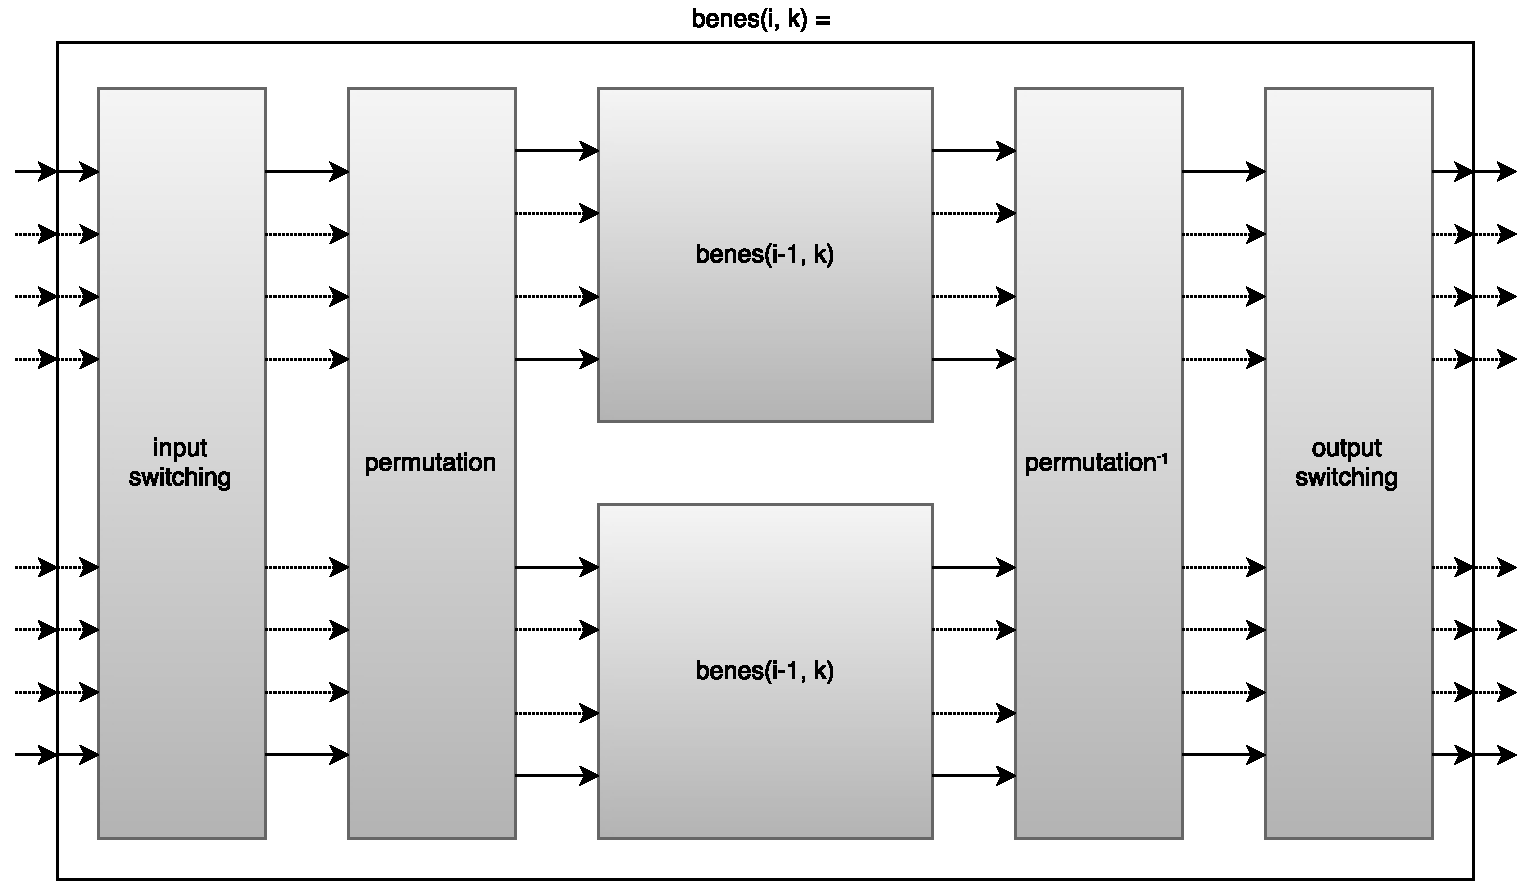
\includegraphics[width=0.9\linewidth]{benes_recursion.pdf}
	\end{center}
\end{frame}

\begin{frame}
	\frametitle{Benes Network: Banyan Stalling Switch}
	\begin{center}
		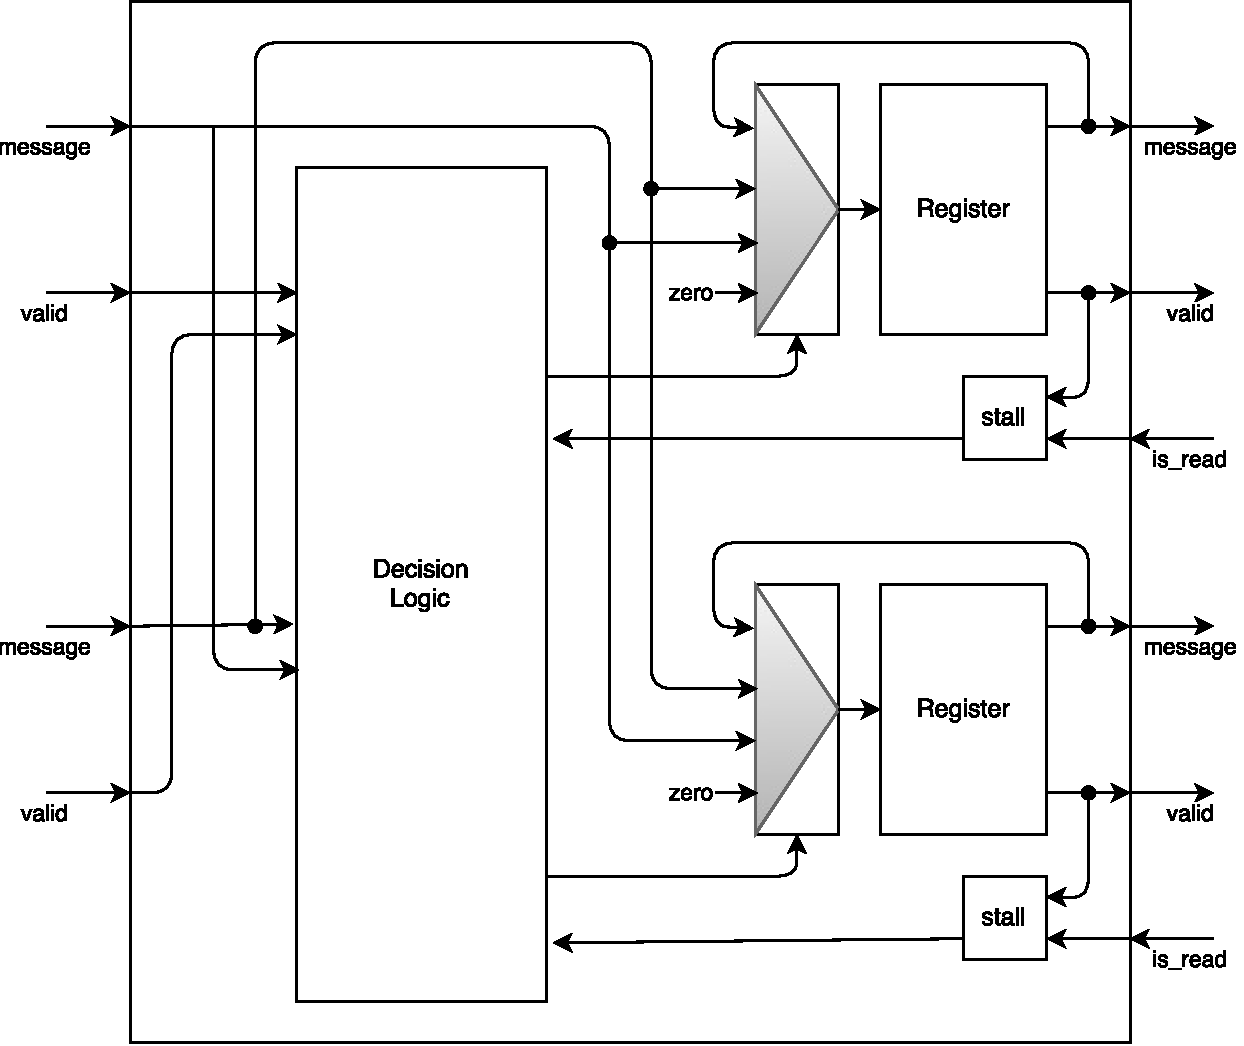
\includegraphics[width=0.7\linewidth]{banyan_stall_switch.pdf}
	\end{center}
	\begin{itemize}
		\item Fixed route for each packet, based on bit $k - i$.
	\end{itemize}
\end{frame}
	
\begin{frame}
	\frametitle{Benes Network: Companions}
	\begin{center}
		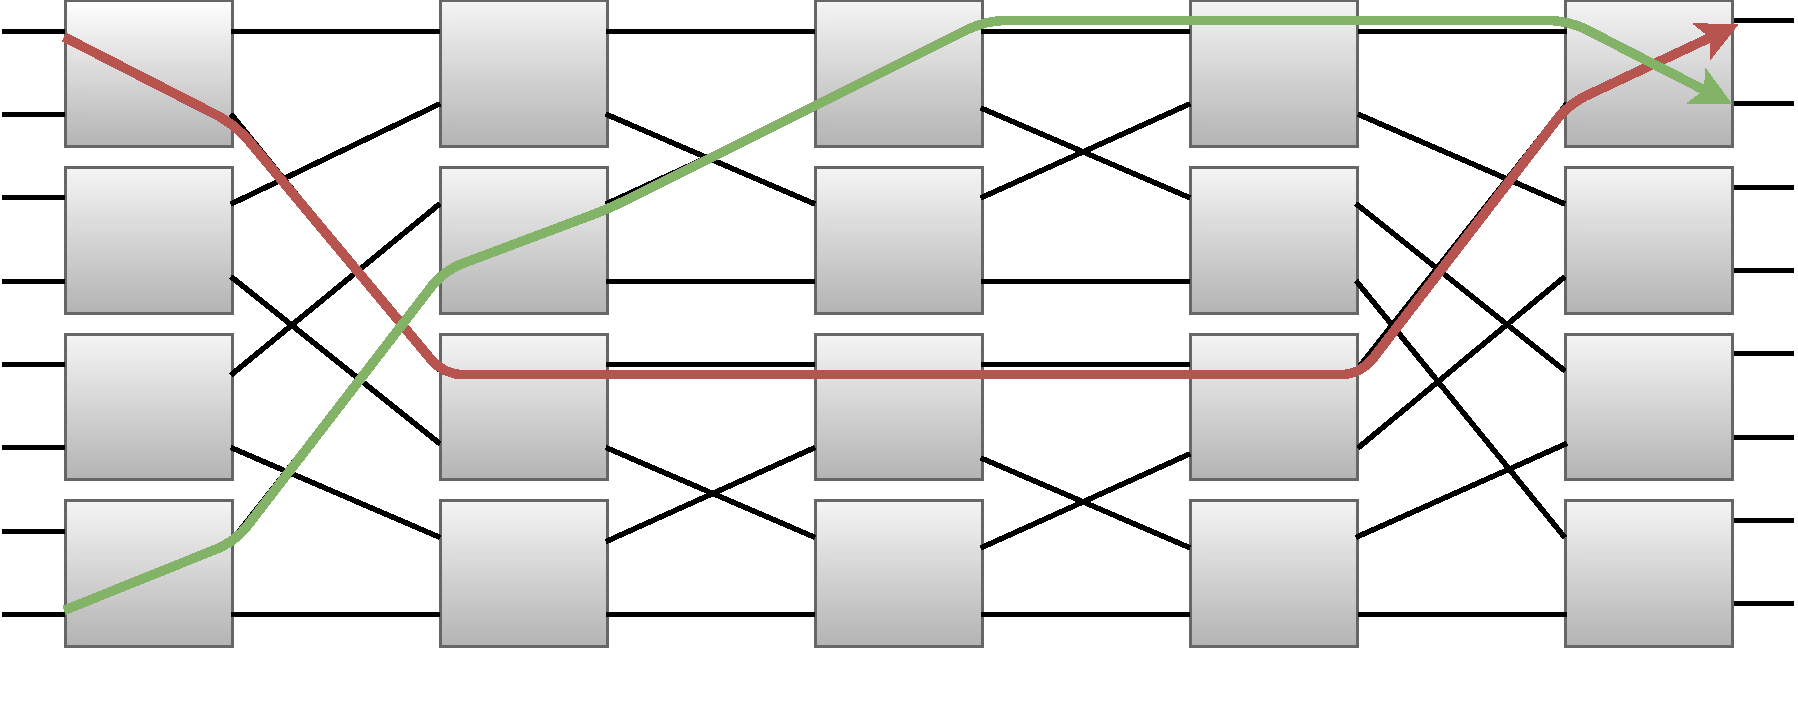
\includegraphics[width=0.9\linewidth]{benes_companions.pdf}
	\end{center}
	\begin{itemize}
		\item Concept by Tripti
	\end{itemize}
\end{frame}

\begin{frame}
	\frametitle{Benes Network: Input Column}
	\begin{center}
		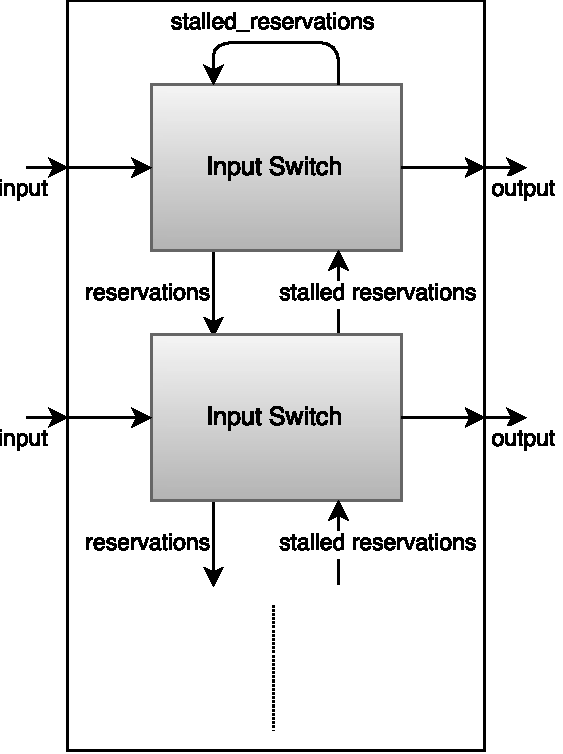
\includegraphics[width=0.3\linewidth]{benes_input_column.pdf}
	\end{center}
	\begin{itemize}
		\item Circuit depth of $O(n)$ $\Rightarrow$ slow
	\end{itemize}
\end{frame}
	
\begin{frame}
	\frametitle{Benes Network: Input Switch}
	\begin{center}
		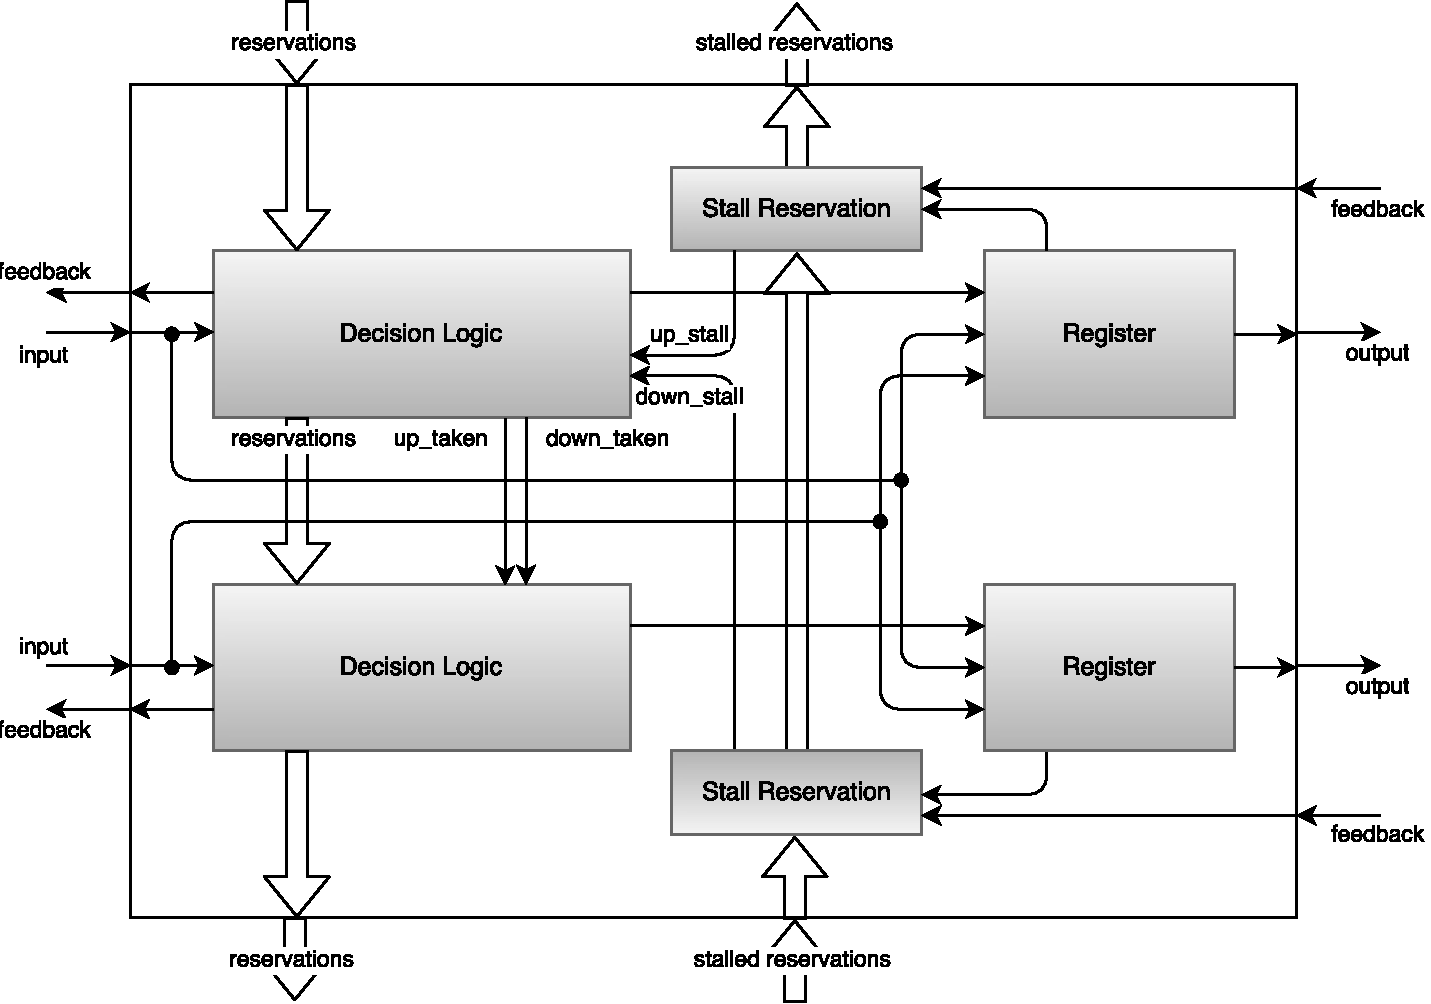
\includegraphics[width=0.8\linewidth]{benes_input_switch.pdf}
	\end{center}
\end{frame}
	
\begin{frame}
	\frametitle{Benes Network: Message Ordering}
	\begin{itemize}
		\item packet from source $s$ and destination $d$
		\item for program order of move instructions $m_n(s_n, d_n) \prec m_{n+1}(s_{n+1}, d_{n+1})$
		\item and delivery order of network $m_n \lhd m_k$
		\item input buffers require:\\
		      $(m_n(s_n, d_n) \prec m_k(s_k, d_k)) \wedge (s_n = s_k \wedge d_n = d_k) \\
		      \Rightarrow (m_n(s_n, d_n) \lhd m_k(s_k, d_k))$
		
		\item Possible stalling and recursive structure $\Rightarrow$ no guarantee so far
		\item (packets with same source and destination might overtake each other)
	\end{itemize}
\end{frame}
	


\section{Memory and Fucntion Units}
  

\begin{frame}
	\frametitle{Functional Units}
	\itemize{
		\item Functional units (FU) are the fundamental processing elements in SCAD architecture
		\item Each FU stores its input operands and output result in buffers
		\item New operations can be added into processor with minimal amount of micro-architectural design effort
		\item In current stepping level, there are two classes of FUs : ALU and memory
	}
\end{frame}


\begin{frame}
\frametitle{Functional Units : ALU}
	\includegraphics[width=\linewidth,height=0.9\textheight,keepaspectratio]{alu_fu.png}
\end{frame}

\begin{frame}
\frametitle{Functional Units : ALU}
	\itemize{
			\item ALU FUs include two buffers for operands and one FIFO buffer for result
			\item Operation to be performed can easily be realized by implementing the well-defined
			ALU operation interface
			\item Single-cycle, multi-cycle or pipelined operations can be added into 
			processor, resulting in easy expansion of ISA !
		}
\end{frame}

\begin{frame}
\frametitle{Functional Units : Memory}
\begin{columns}
\begin{column}{0.48\textwidth}
	\begin{figure}[htbp]
		\centering
		\def\svgscale{0.40}
		\input{figures/load_fu.pdf_tex}
		\caption{Load FU}
		\label{fig:load_fu} 
	\end{figure}
\end{column}
\begin{column}{0.60\textwidth}
	\begin{figure}[htbp]
		\centering
		\def\svgscale{0.28}
		\input{figures/store_fu.pdf_tex}
		\caption{Store FU}
		\label{fig:store_fu} 
	\end{figure}
\end{column}
\end{columns}
\end{frame}

\begin{frame}
		\frametitle{Functional Units : Memory}
\begin{columns}
	\begin{column}{0.48\textwidth}
		\itemize{
			\item Memory is divided into banks, where each bank is accessed by a 
			load/store FU pair
			\item Bank controller serializes accesses to banks by competing load/store
			operations : writes are given precedence
			\item Due to asynchronous data movement, enforcing even a slight consistency
			model seems hard (not formally, but implementation-wise)
		}
	\end{column}
	\begin{column}{0.60\textwidth}
		\begin{figure}[htbp]
			\centering
			\def\svgscale{0.20}
			\input{figures/memory_top.pdf_tex}
			\caption{Top-level memory architecture}
			\label{fig:mem_top} 
		\end{figure}
	\end{column}
\end{columns}	
	


\end{frame}
  
\section{Challenges}
  \begin{frame}
  
\end{frame}
  
\section{Future Work}
  \begin{frame}
  
\end{frame}
  
\end{document}
